\documentclass[11pt]{article}
\usepackage[paperwidth=12cm, paperheight=18cm, margin=1cm]{geometry}
\usepackage{amsmath, tikz}
\pagestyle{empty}

\begin{document}
\begin{center}
  {\LARGE\bfseries The Coupon Collector}\\[4pt]
  {\large How many packs to finish the album?}
\end{center}

Each pack holds one random sticker out of \(n\).
How many packs until you have them all?

\section*{Each new sticker gets harder}
After collecting \(i\) stickers, a new one shows up with
probability \(\frac{n-i}{n}\), so you wait \(\frac{n}{n-i}\) packs:
\[
  E[T] = \sum_{i=0}^{n-1} \frac{n}{n-i}
  = n \left(1 + \frac12 + \dots + \frac1n\right) = n H_n
\]
\[
  E[T] \approx n \ln n + 0.577\, n
\]

\begin{center}
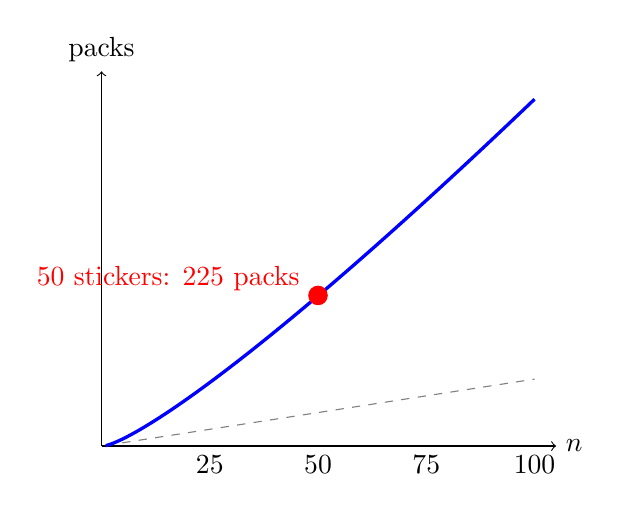
\begin{tikzpicture}[xscale=0.055, yscale=0.0085]
  \draw[->] (0,0) -- (105,0) node[right] {$n$};
  \draw[->] (0,0) -- (0,560) node[above] {packs};
  \draw[gray, dashed, domain=1:100] plot (\x, \x);
  \draw[blue, very thick, domain=1:100, samples=100]
    plot (\x, {\x*ln(\x) + 0.577*\x});
  \foreach \x in {25, 50, 75, 100} \node[below] at (\x,0) {\x};
  \node[circle, fill=red, inner sep=2.5pt] at (50,225) {};
  \node[red, left] at (48,250) {50 stickers: 225 packs};
\end{tikzpicture}
\end{center}

The last sticker alone takes \(n\) packs on average:
as many as the whole first half of the album.
\end{document}
